

%documentclass[a4paper,12pt]{report}
%\begin{document}
%\title{\color{magenta}\underline {Assignment $N^o 1$}}
%\author{Electronica III}
%\author{\color{teal}Group 2}
%\date{\color{blue}\today} %ver si dejar la de today o poner fecha fija que sea August 2018
%\pagenumbering{arabic}

%\maketitle

%EXCERCISE 1 :)

\section{\color{olive}Excercise 1: Resolution and Range of a Fixed-Point Binary Representation}

\subsection{\color{purple}What is the Fixed-Point Binary Representation}
A fixed-point number has an integer part and a fractional part separated by a decimal point with a fixed position, as shown below:
$$ (Integer Part).(Fractional Part)$$
The integer part is formed by $n$ bits and the fractional part is formed by $m$ bits.
$$ (bit \#1\ \ \ bit \#2\ \ \ ...\ \ \ bit \#n).(bit \#1\ \ \ bit \#2\ \ \ ...\ \ \ bit \#m)$$

\subsection{\color{purple}What is Resolution and Range}
\subsubsection{\color{red}Resolution}
The resolution of a number using the fixed point representation is the smallest unit that can be handled with it.
Given a fixed-point number with $m$ fractional bits, the resolution is $2^- $$^m$. %Importante! Ver acá como puse el 2 elevado a la -m, para futuras veces.
\subsubsection{\color{red}Range}
The range is the difference between the biggest value that can be obtained with the fixed-point representation of a number with $n$ bits in the integer part and with $m$ bits in the fractional part, and the smallest number that can be represented.
%ver de poner la ecuacion matematica que permite obtener el range.

\subsection{\color{purple}Using this Program}
\subsubsection{\color{orange}Input}
Three arguments must be entered through Command Line, separated by one or more spaces:
\begin{enumerate}
\item  1 (indicating that the numeric representation of the binary number is signed) or 0 (indicating that the representation is unsigned).
\item $n$: A possitive integer (indicating the number of bits that correspond to the integer part of the number, which appears before the decimal point).
\item  $m$: A possitive integer (indicating the number of bits that correspond to the fractional part of the number, which appears after the decimal point).
Important: $n$ and $m$ are restricted to be less than or equal to 1000.
\end{enumerate}
{\color{cyan}For example: "0 1 1"}.

\subsubsection{\color{orange}Output}
The result of this program is the resolution and range of the number that has $n$ digits in the integer part and $m$ digits in the fractional part. If any of the input requirements is not respected, an error message is printed to the user.

\begin{figure}[h!]
\centering
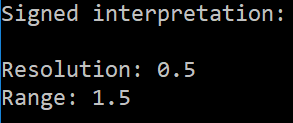
\includegraphics[scale=1]{../E1TP1/ejemploOutput}
\caption{\color{cyan}Output corresponding to the example input $"0\ 1\ 1"$.}
\label{image output}
\end{figure}

\subsection{\color{purple}Testing the Program}
The program was tested with the following cases and worked as expected:
\subsubsection{\color{orange}Inputs that should work}
1 1 0
1 0 1
0 0 1
1 0 0 
0 0 0 
1 12 0
1 1    1
1 3          1
1          3     1
0 1000 1000
0 1000 00000001
0 000 00000001
\subsubsection{\color{orange}Inputs that should not work}
1 1 -1
1 1
0 1000 1001
00 100 1
01 100 1
0 100M 1
\subsection 

%HACEEEEEEEEEEEEEEEEEEEEEEEEEEEEEEEEEEEEEEEEEEEER ESTA PARTEEEEEEEEEEEEEEEEEEEEEEEEEE

%\end{document}


%Información usada:

% beginners guide to latex:
% http://www.docs.is.ed.ac.uk/skills/documents/3722/3722-2014.pdf

% fixed point mathematics:
%http://fileadmin.cs.lth.se/cs/Education/EDA075/notes/mgh_appA_fixed.pdf
